\documentclass[12pt]{report} %fuente a 12pt

% MÁRGENES: 2,5 cm sup. e inf.; 3 cm izdo. y dcho.
\usepackage[
a4paper,
vmargin=2.5cm,
hmargin=3cm
]{geometry}

% INTERLINEADO: Estrecho (6 ptos./interlineado 1,15) o Moderado (6 ptos./interlineado 1,5)
\renewcommand{\baselinestretch}{1.15}
\parskip=6pt

% DEFINICIÓN DE COLORES para portada y listados de código
\usepackage[table]{xcolor}
\definecolor{azulUC3M}{RGB}{0,0,102}
\definecolor{gray97}{gray}{.97}
\definecolor{gray75}{gray}{.75}
\definecolor{gray45}{gray}{.45}

% Soporte para GENERAR PDF/A
\usepackage[a-1b]{pdfx}

% ENLACES
\usepackage{hyperref}
\hypersetup{colorlinks=true,
	linkcolor=black, % enlaces a partes del documento (p.e. índice) en color negro
	urlcolor=blue} % enlaces a recursos fuera del documento en azul

\usepackage{pdfpages}

% EXPRESIONES MATEMATICAS
\usepackage{amsmath,amssymb,amsfonts,amsthm}

\usepackage{txfonts} 
\usepackage[T1]{fontenc}
\usepackage[utf8]{inputenc}

\usepackage{tikz}
\usepackage{pgfplots}

\usepackage[spanish, es-tabla]{babel} 
\usepackage[babel, spanish=spanish]{csquotes}
\AtBeginEnvironment{quote}{\small}

% diseño de PIE DE PÁGINA
\usepackage{fancyhdr}
\pagestyle{fancy}
\fancyhf{}
\renewcommand{\headrulewidth}{0pt}
\rfoot{\thepage}
\fancypagestyle{plain}{\pagestyle{fancy}}

% DISEÑO DE LOS TÍTULOS de las partes del trabajo (capítulos y epígrafes o subcapítulos)
\usepackage{titlesec}
\usepackage{titletoc}
\titleformat{\chapter}[block]
{\large\bfseries\filcenter}
{\thechapter.}
{5pt}
{\MakeUppercase}
{}
\titlespacing{\chapter}{0pt}{0pt}{*3}
\titlecontents{chapter}
[0pt]                                               
{}
{\contentsmargin{0pt}\thecontentslabel.\enspace\uppercase}
{\contentsmargin{0pt}\uppercase}                        
{\titlerule*[.7pc]{.}\contentspage}                 

\titleformat{\section}
{\bfseries}
{\thesection.}
{5pt}
{}
\titlecontents{section}
[5pt]                                               
{}
{\contentsmargin{0pt}\thecontentslabel.\enspace}
{\contentsmargin{0pt}}
{\titlerule*[.7pc]{.}\contentspage}

\titleformat{\subsection}
{\normalsize\bfseries}
{\thesubsection.}
{5pt}
{}
\titlecontents{subsection}
[10pt]                                               
{}
{\contentsmargin{0pt}                          
	\thecontentslabel.\enspace}
{\contentsmargin{0pt}}                        
{\titlerule*[.7pc]{.}\contentspage}  


% DISEÑO DE TABLAS.
\usepackage{multirow} % permite combinar celdas 
\usepackage{caption} % para personalizar el título de tablas y figuras
\usepackage{floatrow} % utilizamos este paquete y sus macros \ttabbox y \ffigbox para alinear los nombres de tablas y figuras de acuerdo con el estilo definido. Para su uso ver archivo de ejemplo 
\usepackage{array} % con este paquete podemos definir en la siguiente línea un nuevo tipo de columna para tablas: ancho personalizado y contenido centrado
\newcolumntype{P}[1]{>{\centering\arraybackslash}p{#1}}
\DeclareCaptionFormat{upper}{#1#2\uppercase{#3}\par}

% Diseño de tabla para ingeniería
\captionsetup[table]{
	format=upper,
	name=TABLA,
	justification=centering,
	labelsep=period,
	width=.75\linewidth,
	labelfont=small,
	font=small,
}

% DISEÑO DE FIGURAS.
\usepackage{graphicx}
\graphicspath{{img/}} %ruta a la carpeta de imágenes

% Diseño de figuras para ingeniería
\captionsetup[figure]{
	format=hang,
	name=Fig.,
	singlelinecheck=off,
	labelsep=period,
	labelfont=small,
	font=small		
}

% NOTAS A PIE DE PÁGINA
\usepackage{chngcntr} %para numeración contínua de las notas al pie
\counterwithout{footnote}{chapter}

% LISTADOS DE CÓDIGO
% soporte y estilo para listados de código. Más información en https://es.wikibooks.org/wiki/Manual_de_LaTeX/Listados_de_código/Listados_con_listings
\usepackage{listings}
\setlength{\parindent}{0em}


% definimos un estilo de listings
\lstdefinestyle{estilo}{ frame=Ltb,
	framerule=0pt,
	aboveskip=0.5cm,
	framextopmargin=3pt,
	framexbottommargin=3pt,
	framexleftmargin=0.4cm,
	framesep=0pt,
	rulesep=.4pt,
	backgroundcolor=\color{gray97},
	rulesepcolor=\color{black},
	%
	basicstyle=\ttfamily\footnotesize,
	keywordstyle=\bfseries,
	stringstyle=\ttfamily,
	showstringspaces = false,
	commentstyle=\color{gray45},     
	%
	numbers=left,
	numbersep=15pt,
	numberstyle=\tiny,
	numberfirstline = false,
	breaklines=true,
	xleftmargin=\parindent
}

\captionsetup[lstlisting]{font=small, labelsep=period}
% fijamos el estilo a utilizar 
\lstset{style=estilo}
\renewcommand{\lstlistingname}{\uppercase{Código}}

\pgfplotsset{compat=1.17} 
%-------------
%	DOCUMENTO
%-------------

\begin{document}
\pagenumbering{roman} % Se utilizan cifras romanas en la numeración de las páginas previas al cuerpo del trabajo
	
%----------
%	PORTADA
%----------	
\begin{titlepage}
	\begin{sffamily}
	\color{azulUC3M}
	\begin{center}
		\begin{figure}[H] %incluimos el logotipo de la Universidad
			\makebox[\textwidth][c]{
\includegraphics[width=16cm]{Portada_Logo.png}}
		\end{figure}
		\vspace{2.5cm}
		\begin{Large}
			Grado en Ingeniería Informática\\			
			2020-2021\\
			\vspace{2cm}		
			\textsl{Apuntes}\\
			\bigskip
		\end{Large}
		 	{\Huge Diseño de Sistemas Interactivos}\\
		 	\vspace*{0.5cm}
	 		\rule{10.5cm}{0.1mm}\\
			\vspace*{0.9cm}
			{\LARGE Jorge Rodríguez Fraile\footnote{\href{mailto:100405951@alumnos.uc3m.es}{Universidad: 100405951@alumnos.uc3m.es}  |  \href{mailto:jrf1616@gmail.com}{Personal: jrf1616@gmail.com}}}\\ 
			\vspace*{1cm}
	\end{center}
	\vfill
	\color{black}
		
\includegraphics[width=4.2cm]{img/creativecommons.png}\\
		Esta obra se encuentra sujeta a la licencia Creative Commons\\ \textbf{Reconocimiento - No Comercial - Sin Obra Derivada}
	\end{sffamily}
\end{titlepage}

%----------
%	ÍNDICES
%----------	

%--
% Índice general
%-
\tableofcontents
\thispagestyle{fancy}

%--
% Índice de figuras. Si no se incluyen, comenta las líneas siguientes
%-
\listoffigures
\thispagestyle{fancy}

%--
% Índice de tablas. Si no se incluyen, comenta las líneas siguientes
%-
\listoftables
\thispagestyle{fancy}

%----------
%	TRABAJO
%----------	
\clearpage
\pagenumbering{arabic} % numeración con números arábigos para el resto de la publicación	


%----------
%	COMENZAR A ESCRIBIR AQUI
%----------	


\section{Información}
\begin{quote}
Teorías: Elena Márquez Segura (Coordinadora) elena.marquez@uc3m.es

Prácticas: Pablo Acuña pacua@inf.uc3m.es
\end{quote}

\section{Recursos}

\href{https://www.acontracorrientech.com/claves-para-entender-angular-que-es-y-como-se-utiliza/}{Claves para entender Angular - Qué es y cómo se utiliza este framework}

\href{https://www.acontracorrientech.com/guia-practica-del-databinding-en-angular/}{Guía de iniciación al data binding en Angular | Qué es y cómo se utiliza}

\section{Cuestionarios}

\subsection{Test 1}

\textbf{El contexto de diseño caracteriza\ldots{}}
\begin{itemize}
  \item \ldots{} la situación/práctica/fenómeno/actividad para la que se va a diseñar
\end{itemize}

\textbf{Verdadero o Falso: El contexto de diseño considera, entre otras cosas, quiénes son los/as usuarios/as, sus características, necesidades, deseos\ldots{}}
\begin{itemize}
  \item Verdadero
\end{itemize}

\textbf{Obtener consentimiento por parte de los/as participantes (usuarios/as)\ldots{}}
\begin{itemize}
\item Todas las anteriores (participantes y entrevistados)
\end{itemize}

\textbf{En entrevistas y cuestionarios, las preguntas cerradas tienen sentido cuando\ldots{}}
\begin{itemize}
\item \ldots tenemos claro el foco y objetivo de la investigación
\end{itemize}

\textbf{En general, esta es una pregunta correcta en una entrevista: ``¿Qué problemas tienes con este producto?''}
\begin{itemize}
  \item Falso
\end{itemize}

\textbf{En general, esta es una pregunta correcta en una entrevista: ``¿crees que el producto debería ser más pequeño y barato?''}
\begin{itemize}
\item Falso
\end{itemize}

\newpage

\textbf{Marca todas las correctas. Un ``Contextual Inquiry''\ldots{}}
\begin{itemize}
  \item \ldots{} se puede considerar una técnica etnográfica
  \item \ldots{} es una técnica de observación directa en la que el/la investigador/a mantienen un rol activo, preguntando a medida que van observando
\end{itemize}

\textbf{Un Experience Sampling Method (ESM) es\ldots{}}
\begin{itemize}
  \item \ldots{} es una técnica cualitativa de observación indirecta parecida al diario, en la que se mandan prompts o recordatorios a los/as participantes
\end{itemize}

\textbf{Marca todas las respuestas verdaderas acerca de Embodied Interaction}
\begin{itemize}
\item \ldots{} se puede referir a cualquier sistema interactivo, desde móviles y ordenadores, hasta videojuegos de movimiento
\item \ldots{} es un enfoque de diseño y estudio de sistemas interactivos que se centra en, y saca partido de cómo las personas entienden y actúan en el terreno físico y social
\end{itemize}

\textbf{Señala todas las respuestas correctas acerca del análisis de datos}
\begin{itemize}
  \item Se pueden tener datos cualitativos y hacer análisis cuantitativos y viceversa
  \item En análisis cuantitativo, podemos encontrarnos variables cualitativas y variables numéricas
\end{itemize}

\chapter{Web Components}

\textbf{Evolución de los paradigmas de programación:}

\begin{itemize}
  \item Programación monolítica.
  \item Programación procedimental -- Encapsula datos locales.
  \item Programación POO -- Encapsula datos y funciones.
  \item Programación conducida por eventos -- Facilita GUI a partir de componentes.
\end{itemize}

\textbf{Paradigmas programación web}: Ha seguido una evolución parecida.

\begin{itemize}
\item HTML Monolítico (la web es estática)
\item HTML (datos + estructura) + CSS (estilo gráfico) + JS (comportamiento)
\item Antes se mandaba el HTML completo, pero hoy en día se envía JSON que son más ligeros y transmiten solo datos.
\end{itemize}

\textbf{WEB COMPONENTS (W3C + Google -\textgreater{} web components)}: Para personalizar y facilitar el desarrollo web, se crean:

\begin{itemize}
\item
  \textbf{Custom HTML Components}: Definir nuevas etiquetas.
\item
  \textbf{HTML Template}: Preparados para enmaquetar.
\item
  \textbf{Shadow DOM}: Encapsula elementos DOM.
\item
  \textbf{HTML imports}: Librerías, que permiten modularizar
  aplicaciones.
\end{itemize}

Su uso facilita la programación web y la compatibilidad con cualquier
navegador.

\textbf{Problemas del estándar}: Incompatibilidades entre navegadores y
HMLT imports obsoletos.

\textbf{Frameworks (React/Vue.js/Angular)}

\textbf{Angular}: Tiene una curva de aprendizaje compleja. Es bueno para aplicaciones complejas como intranet, extranet, aplicaciones corporativas. Además, es un Framework completo dirigido a desarrolladores corporativos.

\chapter{Introducción}

\textbf{HCI - Human-Computer Interaction}: Interacción
Persona-Ordenador.

\textbf{IxD - Interaction Design}: Diseño de Interacción.

\textbf{Usability}: Usabilidad.

\textbf{UX - User Experience}: Experiencia de Usuario.

\textbf{UCD - User-centered Design}: Diseño Centrado en el Usuario.

Un buen diseño muy importante para el uso de los sistemas, incluso puede ser cuestión de vida o muerte. En los que un mal diseño tiene consecuencias graves, en estos se usa redundancia y cosas claras. Aunque la mayoría de las veces son problemas cotidianos.

\textbf{Affordance}: Que te dice como hacer, que te permite, que se
ofrece. Gibson(70s) en el entorno medible relacionales, Norman(80s) son
fáciles de percibir y Gaver(90s) perceptibles falsas ocultas.

\begin{itemize}
\item
  \textbf{Secuenciales}: Al realizar una nos lleva a otra. Girar un pomo
  y empujar para abrir.
\item
  \textbf{Anidadas}: Una puerta en un marco, con un pomo. Una dentro de
  otra.

  Ejemplo: Un asa pide tirar y una placa empujar.
  \begin{figure}[H]
	\ffigbox[\FBwidth]
	{\caption{Diagrama affordance}}
	{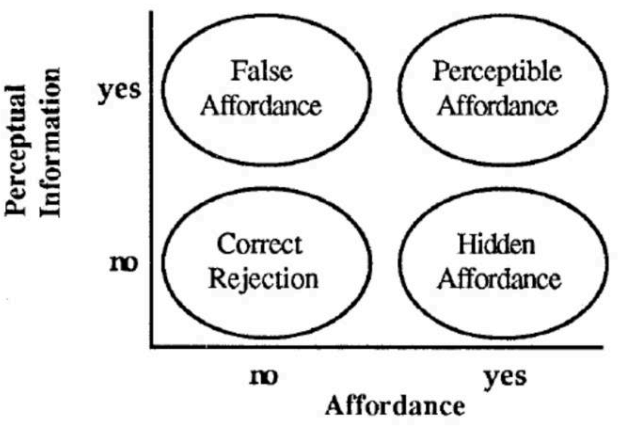
\includegraphics[scale=.4]{Untitled.png}}
\end{figure}
\end{itemize}

\textbf{Mapping}: Coincidencia entre los controles y la representación
física.

\hypertarget{tema-1}{%
\chapter{Tema 1}\label{tema-1}}

\textbf{HCI - Human-Computer Interaction}: Interacción
Persona-Ordenador.

\textbf{IxD - Interaction Design}: Diseño de Interacción.

\textbf{Usability}: Usabilidad.

\textbf{UX - User Experience}: Experiencia de Usuario.

\textbf{UCD - User-Centered Design}: Diseño Centrado en el Usuario.

\textbf{IS - Information Systems}: Sistemas de Información.

\textbf{Sistema Interactivo}: Aquello que reciben datos y realizan una
acción o proceso.

\section{La interfaz}

Medio de interacción y comunicación con los usuarios, que permite enviar
y recibir información.

\textbf{Sistema}: Objeto complejo formado por múltiples partes
relacionadas e interconectadas.

\textbf{Interactivo}: Que permite la interacción.

\textbf{Interacción}: Acción o relación recíproca entre varios objetos.

\section{Diseño de Sistemas
Interactivos}

Campo multidisciplinar que se centra en diseñar el comportamiento de
sistemas con los que interactúan los usuarios y forman parte. Para
apoyarlo en su día a día.

Trata de crear experiencias que aumentan, extienden, mejoran, aporta,
construyen, facilitan la manera en la que la gente trabaja o actúa.
Desarrollar tecnología que sea fácil y agradable de usar para los
usuarios.

Equipos multidisciplinares, hay que tener en cuenta muchos factores para
el diseño centrado en usuario.

\section{Usabilidad vs. Experiencia de
Usuario}

\textbf{Usabilidad}: La eficacia, la eficiencia y la satisfacción de
usuarios determinados alcanzando objetivos concretos en un contexto
determinado.

\textbf{UX}: Percepciones y respuestas resultado del uso (y anticipación
de uso) de un producto, sistema o servicio. En definitiva, todos los
aspectos de la experiencia del usuario al interactuar con un producto,
servicio, entorno o establecimiento.

\section{HCI}

HCI en el inicio, una pequeña muy pequeña del diseño.

Hoy en día, es un campo muy amplio.

Evolución de HCI en olas.

\section{Etapas en HCI -- Olas}

Distintos paradigmas (modelo/superteoria), programa, y de investigación
y diseño. Etapas.

Coexisten, a veces en conflicto, lo que afecta lo que entendemos por
verdad. No está bien definida la frontera o distinción.

\subsection{Primera Ola}

Es el primer paradigma (Harrison): \textbf{Ergonomía y Factores
Humanos}, psicología + inteligencia.

Muy pragmático, ateórico.

\textbf{Metáfora}: Interacción vista como el encaje entre la persona y
la máquina. El objetivo, es que encajen bien para que funcione.

\textbf{Foco}: Identificar problemas concretos en la interacción que
crean mal funcionamiento y desarrollar una solución para que encajen.

\subsubsection{Background}

HCI emerge en \textbf{80s}, \textbf{encaje de persona-maquina}.

Se habla de factores humanos, dimensiones, capacidades, y limitaciones
de usuarios.

\textbf{Influencia}: Ingeniería y psicología trabajando mano a mano.

\textbf{Metáfora}: Mente y computadora como un procesador de información
acoplada.

Investigación en universidades y laboratorios industriales.

\textbf{Tecnología}: WIMP.

\subsubsection{Foco}

\textbf{Trabajo}: Centrado en la oficina, ordenadores de sobremesa.

Trabajo, tareas, productividad. Muy centrada en la máquina.

\textbf{Estudios}: Evaluaciones de sistemas existentes. Análisis de
características de uso en situaciones específicas.

\subsubsection{Teoría}

User friendly -- \textbf{Amigable para el usuario.}

\textbf{De usabilidad}: Útil, eficiente, eficaz, fácil de aprender y
satisfacción.

El \textbf{objetivo es decrementar la carga mental}, reducir el abismo.

\begin{itemize}
\item
  \textbf{Abismo (golfo) de ejecución}: Diferencia entre las acciones
  que el usuario quiere hacer para alcanzar el objetivo y las acciones
  permitidas por el sistema.
\item
  \textbf{Abismo de evaluación}: Diferencia entre lo que esperaba el
  usuario observar y lo que el usuario ve, le requiere más esfuerzo.

  Cuanto más tamaño de abismo, más dificultad de entender.
\end{itemize}

\textbf{Affordances} (Gibson, Norman, Gaver)

\begin{itemize}
\item
  \textbf{Gibson}: Relativas a las capacidades de los actores, no todos
  los perciben, pero son independiente de su percepción, aunque no lo
  veas no quiere decir que no esté.
\item
  \textbf{Norman} las introduce en HCI en relación con el diseño e
  introduciendo el factor de la percepción.

  Cuando está bien hecho, el usuario solo mirando es capaz de
  reconocerlo, sin dibujos, ni etiquetas.
\item
  \textbf{Gaver}: Perceptibles, falsas, ocultas.

  \begin{itemize}
  
  \item
    \textbf{Secuenciales}: Una te da información para hacer otra.

    \begin{itemize}
    
    \item
      \textbf{Anidadas}: Una affordance sirve como contexto de otra.
    \end{itemize}
  \end{itemize}
\end{itemize}

\textbf{Modelo conceptual vs. Modelo mental} (Craik)

\begin{itemize}
\item
  Ideal vs. Realidad
\item
  \textbf{Modelo conceptual}: Como el diseñador lo concibe e implementa.
\item
  \textbf{Modelo mental}: Como piensa el usuario que funciona el
  sistema.
\item
  El diseñador debe basar su modelo conceptual en cómo piensan los
  usuarios, hay que preguntar y usar experiencias en productos previos.
\end{itemize}

\subsubsection{Métodos}

En el laboratorio, experimentos controlados.

Modelos de como la persona realiza una tarea, como GOMS y KLM.

Asume usuarios que saben, ayuda a tomar decisiones de la interfaz y
enfoque reduccionista.

Modelado de factores humanos, especificaciones, guiar y requisitos
rígidos.

\textbf{Testeo sistemático de usabilidad} (Rubin and Chisnell)

\textbf{Utilidad}: Conseguir objetivos.

\textbf{Eficiencia}: Completar tarea en el menor tiempo. Se mide en
tiempo.

\textbf{Eficacia y efectividad}: Completar tarea de manera correcta. Se
mide en ratio de errores.

\textbf{Fácil de aprender}: Se mide en tiempo de aprendizaje.

\textbf{Satisfacción}: Percepción de usuarios, opinión, sentimiento. Se
mide con valores y rangos.

Evaluación de expertos. Heurísticas.

\subsubsection{Contribución y Valores}

Evaluación de sistemas.

Análisis de tareas.

Especificaciones de diseño, importante para fases posteriores ciclo de
diseño.

El diseño, no están importante, es un vehículo.

Investigación en HCI.

\subsection{Segunda Ola}

\subsubsection{Background}

1990s

Se pasa de usuarios a personas, productos a sistemas, usuarios novatos a
usuarios más experimentados, de individuos a grupos y de laboratorios a
entorno de trabajo.

Se mira a la interacción más que al computador.

\textbf{Contexto}: Mira al espacio de trabajo y la gente alrededor.

\textbf{De análisis a Diseño}: De trazar requisitos de usuarios a
prototipado iterativo, de usuarios al final a diseño centrado en usuario
(UCD)

\subsubsection{Teoría}

Situaciones reales y complejas en el entorno de trabajo.

\textbf{Importancia del contexto.}

\textbf{Coordinación de acción conjunto}: Coincidencia, colaboración y
cooperación.

\paragraph{Situated Action o Acción situada (Rogers)}

La interacción se entiende situada como atada al ahora y aquí en ese
contexto.

La gente no son maquinas, no siguen procedimientos a rajatabla.

Los planes cambian en interacción con el entorno, cambia según vamos
avanzando por que vamos viendo el progreso.

\textbf{Perspectiva interaccionista y ecológica}: Relación entre
estructuras de acción y los recursos ofrecidos por el contexto físico y
social.

\textbf{Objetivo}: El diseño de interacción debe apoyar la acción
situación (la acción que suele pasar en un lugar determinado) y la
creación de significado (según la circunstancia).

\textbf{Estudio:}

\begin{itemize}
  \item Escenarios de trabajo.
  \item Contraste entre lo que la gente hace vs. Lo que se supone que tienen que hacer.
  \item Métodos etnográficos.
\end{itemize}

\textbf{Nos quedamos con:}
 \begin{itemize}
   \item Para diseñar tecnología para el trabajo, hay que considerar los detalles de las prácticas de trabajo.
   \item Importancia de trabajo de campo (in the wild) para entender el contexto y la situación.
 \end{itemize}


\textbf{Critica}: Muy centrado en lo particular, difícil generalizar.

\paragraph{Distributed Cognition o Cognición
Distribuida}

De ciencias cognitivas. Cognición y conocimiento no están confinados en
el individuo, si no en su entorno.

``La mente está en el mundo'' distribuido a través de un ``sistema
cognitivo''

\textbf{Usos}: Estudio de trabajos que cuentan con espacio como lugar de
cognición.

\textbf{Análisis}: interacción entre individuos, el medio
representacional, el espacio donde la actividad tiene lugar.

\textbf{Útil para}: Cambiar diseños para mejorar rendimiento.

\textbf{Examinar (a nivel de evento, muy al detalla):}

\begin{itemize}
  \item La resolución distribuida de problemas.
  \item Medios/canales de comunicación.
  \item Rol de comunicación verbal y no verbal.
  \item Mecanismo de coordinación.
  \item Como la información y el conocimiento se comparte, acceder, propaga\ldots{}
  \item Como se coordinan las unidades distribuidas.
\end{itemize}


\textbf{Anotar}: Incidente, problemas, caminos de
información/comunicación.

\textbf{Resultados}: Explicación de interdependencias complejas entre
los elementos del sistema cognitivo.

\textbf{Critica}: No rápido y sucio (``quick and dirty''),
receta\ldots{}

\subsubsection{Métodos}

Proactivos.

User-Centered Design Processes (Norman and Draper)

\textbf{Participatory Design o Diseño Participativo}: Democratizar el
proceso de diseño, el usuario participa en el diseño.

Investigación y diseño contextual.

\textbf{Análisis}: Sociología, antropología, etnometodología. Trabajos
de campo, Técnicas observacionales y Microanálisis.

\subsubsection{Contribución y Valores}

\textbf{Emergencia CSCW (Computer Supported Cooperative Work)}: Extiende
el foco de la diada persona-computador a grupos de trabajo. Centrado en
tareas colaborativas/cooperativo.

Perspectiva Situada.

Diseño como disciplina, Design Science.

Importancia de los usuarios en el proceso de diseño, UCD.

\subsection{Tercera Ola}


\subsubsection{Background}

2000s

Los Usuarios pasan a llamarse Actores o Participantes.

El contexto y el campo de aplicación se amplía, del lugar de trabajo al
hogar o calle, del trabajo al día a día.

Mas allá del rendimiento, y la información sobre la vida humana.

\textbf{Elementos en la vida humana}: Cultura, Emociones, Experiencia.

La tecnología también amplia alcance, tecnología móvil, ubica,
ambiental, tangible\ldots{} y espacios híbridos.

\subsubsection{Teoría}

De lo cognitivo a lo emocional. Experiencia estética, desde una
perspectiva pragmática/cultural/fenomenológica.

\textbf{Embodied Interaction}: Es la creación, manipulación y
compartición de significado mediante la interacción con artefactos
físicos. Enfoque de diseño que tienen muy en cuenta aspectos y contextos
físico y sociales. Inspirado en Social Computing y Tangible Computing.
Aunque se usa para hablar de sistemas gestuales y de movimiento NO
existe una interacción que no sea embodied, pero hay que ver como los
usamos.

\textbf{Embodied phenomena}: Que nos lo encontramos en el mundo físico
más que abstracto.

\textbf{Embodiment (encarnación, la corporalidad):} La manera en la que
nos encontramos la realidad física y social en el mundo de todos los
días. Significa poseer y actuar mediante una manifestación física en el
mundo.

Cambio de perspectiva.

Revisión de compromisos hechos hace 70 anos. Primaba minimizar tiempo de
computación, primaba la computación sobre los usuarios.

\textbf{Nuevas tecnologías:} Móviles, relojes, gafas, coches\ldots{}

\textbf{El problema:} Esto empeora los efectos de esos compromisos.

Necesitamos nuevas maneras de interactuar con computadores, que se
ajusta mejor a nuestras necesidades, habilidades, valores\ldots{}

Para una nueva interacción y experiencia, se explota nuestras habilidades
y familiaridad con objetos del día a día, para que la computación se
manifieste como si fuera un objeto del día a día.

\subsubsection{Métodos}

Más allá de los usuarios. Es un enfoque más explicativo.

\textbf{Diseño en el centro:}

\begin{itemize}
\item
  \textbf{Design Thinking:} Inspirado en prácticas, en artes, en diseño.
  Pensamiento ``no racional'' en el sentido de ``no científicos''.
  Pensar fuere de la caja, out of the box. Innovación, se centra en lo
  que aún no existe.
\item
  \textbf{Embodied design Methods:} Métodos que usan corporalidad de los
  diseñadores y usuarios.
\item
  \textbf{Research through Design (RtD):} Conocimiento a través del
  diseño.
\end{itemize}

\subsubsection{Contribución y Valores}

De centrarse en la información, a centrarse en la acción, en las
sensaciones, emociones.

\textbf{Conceptos:} Sentir y significado, embodied.

\textbf{Artefactos:} Propósitos sociales, y personales + profundos.

\textbf{Énfasis estético:} Emoción, sensación, disfrute, placer, social,
playful, embodied, divertido\ldots{}

Embodied Interaction, ``engagement'' físico y social.

Métodos que tienen el diseño en el centro.

De interpretación objetivo a subjetiva, de individuo a colectivo.

\newpage

\section{User Centered Design (UCD)}

\begin{figure}[H]
	\ffigbox[\FBwidth]
	{\caption{Diagrama proceso UCD}}
	{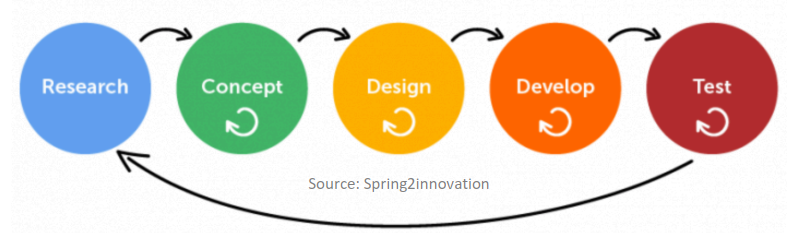
\includegraphics[scale=.4]{image-20210312134547277.png}}
\end{figure}

Proceso iterativo de diseño, centrado en los usuarios.

Involucrados a través de todo el proceso de diseño.

Múltiples técnicas para entender sus necesidades, deseos,
valores... Investigativas y Generativas.

\textbf{Objetivo}: Crear experiencias y productos usables, accesibles,
etc.


\subsection{Fases}

\begin{itemize}
\item
  \textbf{Entender el contexto de diseño}: Necesidades, deseos, etc.
  llevan a requisitos y valores de diseño.

  Documentación, Entrevistas, Cuestionarios, Observación y Focus Group.

  Generan Personas, Escenarios y Requisitos
\item
  \textbf{Diseño}.

  Sketch, Paper Prototype, Wireframes, Mockup y Software Prototype.
\item
  \textbf{Evaluación vs. Contexto de diseño: usuarios y requisitos.}

  Formativa//Sumativa, En el lab//In the wild, Usabilidad, Métodos de
  inspección, Experimentos, Entrevistas y observaciones.
\end{itemize}

El diseño centrado en usuarios es un proceso caro, requiere mucho tiempo
hablar con personas, producir prototipos y demás fases del proceso. Pero
merece la pena este coste para diseñar sistemas bien.

\subsection{Ventajas}

Diseñador no es lo mismo que Usuarios.

Problemas, necesidades y deseos que vemos no son lo mismo que los que
tiene el usuario.

Contacto con usuarios, \textbf{aumenta la empatía y que se lleve a cabo
un diseño ético}, que respete las necesidades y prácticas de los
usuarios.

Involucrar a usuarios, hace que sea \textbf{más probable que se cumplan
sus necesidades y requisitos}, lo que hace que tengamos más ventas y
menos problemas de atención al cliente.

Pensar en el contexto y tareas específicas del usuario, hace que haya
\textbf{menor error humano y más seguridad}, se tienen en cuenta más
factores que hay cuando se usa el sistema.

\chapter{Tema 2: Primera fase UCD}

\section{Contexto de Diseño}

Conocer al usuario, sus objetivos, características y contexto.

\textbf{Caracterización de la situación, fenómeno, práctica o actividad
para la que se va a diseñar.}

Quienes son los usuarios, sus objetivos, necesidades, actividades que
realizan, espacio donde tiene lugar y que recursos tiene.

\section{Técnicas básicas de recogida de
datos}

Sirven para describir y acotar el contexto.

\subsection{Investigación Previa}

\textbf{Estudio de documentación}

Manuales, legislación, datos estadísticos del gobierno, etc.

Feedback directo, mediante logs, muestras de email, investigación de
mercado (da información actual), user testing o libro blanco. Redes
sociales o Reviews.

\textbf{State of the art (``lo último'')} Ver lo que hay

Producto que la gente usa en nuestro contexto de diseño. Para la
innovación es descubrir la oportunidad.

\subsection{Claves para Recogida de
Datos}

\textbf{El objetivo} es entender mejor el espacio de diseño.

Se \textbf{condiciona} por la técnica, los datos, el análisis, etc.

Es importante \textbf{formularla más o menos formalmente}, se parte de
una manera más general y se va concretamente.

\textbf{Identificar a los participantes}, para los usuarios que vamos a
diseñar.

Hay que coger muestras del conjunto de participantes, no se puede
acceder a todos.

\newpage

Tipos de muestras:

\begin{itemize}

\item
  \textbf{Muestreo probabilístico:}

  \begin{itemize}
  
  \item
    \textbf{Aleatorio}: Un número aleatorio de participantes.

    
    \item
      \textbf{Estratificado}: Grupo representativo.
  \end{itemize}
\item
  \textbf{Muestreo no probabilístico:}

  \begin{itemize}
  
  \item
    Conveniencia: Los que haya o se ofrezcan.

    
    \item
      Voluntarios.
  \end{itemize}
\end{itemize}

\textbf{Relación con participantes}

Debe ser \textbf{clara y profesional}, informar de quién somos, que
estamos estudiando, que haremos con la información y como se va a tratar
sus datos.

\textbf{Consentimiento}: Proteger \textbf{participantes e investigador}.

Incentivos, por conveniencia para que haya más participantes, ya que
puro voluntario es más difícil.

\textbf{Triangulación}: Investigación de un fenómeno desde al menos dos
perspectivas:

\begin{itemize}
\item
  De datos, usando distintas fuentes.
\item
  De investigadores.
\item
  \textbf{Metodológica}: uso de distintas técnicas de recogida de datos.
\end{itemize}

Que sea metodológica.

\textbf{Estudio piloto.}

\textbf{Versión reducida} del estudio.

\textbf{Se prueba esa versión antes del estudio principal}, se realizan
preguntas más dirigidas a saber si está bien el cuestionario qua a las
propias respuestas, se realiza de forma iterativa. Identifica problemas
y se aprende de errores. Sobre el protocolo a seguir, equipo,
instrucciones, preguntas, cuestionarios.

\subsection{Captura de Datos}

Importante para análisis posterior.

Algunas formas de recogida de datos se \textbf{auto-documentan}, es decir que los datos indican todo, no hay que interpretarlos.

Muchas otras no, como la observación directa, entrevistas\ldots{}

\newpage

\textbf{Técnicas}

\begin{itemize}
\item
  \textbf{Anotaciones de campo:}

  Es una técnica más resumida con menor número de detalles.

  \textbf{Ventajas}: Más flexible, menos logística y menos intrusivo.

  \textbf{Desventajas}: Más difícil de escribir y preguntar, observar,
  \ldots{}
\item
  \textbf{Grabación de audio:}

  Alternativa a las anotaciones, que se pueden transcribir
  posteriormente.

  Facilita la documentación.
\item
  \textbf{Grabación de video:}

  Proporciona captura visual y auditiva.

  El problema es que requiere más planificación y logística, como
  cámaras, localización o baterías, y es más intrusivo.
\item
  \textbf{Audio y video: Sin tratar (raw data)}

  Se puede consultar en cualquier momento y revisar.
\end{itemize}

\subsection{Entrevistas}

Consiste en un entrevistador \textbf{preguntando a usuarios con un
objetivo}. Normalmente de forma \textbf{síncrona}.

\textbf{Tipos}, dependiendo del control de entrevistador y libertad de
los participantes:

\begin{itemize}
\item
  \textbf{No estructuradas:} Sin protocolo o preparación.

  Preguntas abiertas, que son explicativas que nos permite extraer
  conocimiento.

  La ventaja es que permite respuestas más profundas y más datos, lo que
  permite entender mejor el contexto de diseño.

  Datos complejos, aunque interrelacionados.
\item
  \textbf{Estructuradas:} Más control.

  Preguntas cerradas (lista de opciones) y predeterminadas, como un
  cuestionario. Preguntas cortas, claras y sencillas.

  Las mismas para todos los participantes.

  Se realizan cuando se tiene un objetivo claro, una serie de preguntas
  específicas y repuestas esperadas.

  Requieren menor tiempo.
\item
  \textbf{Semi-estructuradas}

  Combina de los otros dos tipos.

  Guion con:

  \begin{itemize}
  \item
    Serie de temas a cubrir, y preguntas planificadas.

    \begin{itemize}
    
    \item
      Preguntas específicas de seguimiento o para sonsacar más
      información.
    \end{itemize}

    \textbf{Probing o prompts}, preguntas neutras como: ¿Algo que
    añadir?

    \textbf{Herramientas de apoyo:} Gráficos, imágenes de la
    experiencia.
  \end{itemize}
\end{itemize}

\textbf{Planificación}:

\begin{itemize}

\item
  \textbf{Donde}:

  \begin{itemize}
  
  \item
    \textbf{Online}: Es más cómodo, pero necesita logística extra.
    
    \item
      \textbf{En el sitio:} Se realiza en el entorno de uso por lo que
      se observa el entorno, suscita preguntas.
    \item
      \textbf{Sitio neutro o contexto artificial:} Como un laboratorio.
      La logística está más a mano, pero es más difícil poner en
      situación y contexto artificial.
  \end{itemize}
\item
  \textbf{Protocolo (no intimidar):}

  \begin{itemize}
  
  \item
    \textbf{Introducción}: Quién eres, objetivo, temas éticos,
    consentimiento.

    
    \item
      \textbf{Preguntas demográficas. Preguntas de warm-up.}
    \item
      \textbf{Sesión principal:} Temas y preguntas clave.
    \item
      \textbf{Preguntas de cool-off:} Preguntas finales.
    \item
      \textbf{Cierre}: Espacio para que pregunten, agradecimientos e indicar que ha terminado.
  \end{itemize}
\end{itemize}

\textbf{Desarrollar las preguntas:}

Depende del tipo de entrevista.

\textbf{Evitar}: Preguntas largas, confusas, jerga específica, preguntas
peligrosas que condicionan respuestas (asumir algo, coacción o se les
pueda dar la vuelta), cerradas y binarias sin seguimiento, y preguntas
de doble-cañón (no queda claro a cual responde, porque hay varias
posibles).

La \textbf{documentación}, \textbf{equipo} y material para recoger
datos, \textbf{gestión} de la cita y espacio, y \textbf{realizar la
entrevista}.

\subsection{Cuestionarios}

Consiste en una \textbf{serie de preguntas}. Normalmente de forma
\textbf{asíncrona}.

Para obtener respuestas a preguntas específicas de \textbf{muchos
participantes.}

\textbf{Las preguntas pueden ser:} Preguntas abiertas o cerradas.

\textbf{Ventajas}: Mayor alcance y distribución, más conveniente para
los participantes.

\textbf{Desventajas}: Menor riqueza que una entrevista, aunque similar a
una entrevista estructurada.

\textbf{Diseño}

\begin{itemize}
\item
  \textbf{Estructura:}

  Información acerca del estudio y consentimiento, tiempo estimado de
  realización, instrucciones claras de cómo completarlo.

  Preguntas demográficas (identificar el tipo de persona).

  Preguntas especificas agrupadas por temática.
\item
  \textbf{Orden:} Lógico para facilitar la realización, las preguntas
  más generales primero.

  Distintas versiones para poblaciones distintas.
\item
  \textbf{Estilo}: Compacto, pero no cargado y mostrar el progreso en el
  cuestionario.
\item
  \textbf{Evitar}: Preguntas mal formuladas, preguntas negativas para
  evitar que pueda equivocarse y falta de claridad, ya que no estamos
  aclararlo.
\end{itemize}

\textbf{Formatos}

\begin{itemize}
\item
  \textbf{Check boxes y rangos}. Ejm: O 18 to 21
\item
  \textbf{Rating Scale:}

  \begin{itemize}
  
  \item
    \textbf{Escala semántica diferencial}: Good \_ \_ \_ \_ \_ \_ \_ Bad
    
    \item
      \textbf{Likert}: Normalmente de 5 a 7 puntos, según como preciso
      queremos que sean. Orden consistente. Número par para forzar la no
      neutralidad.
  \end{itemize}
\end{itemize}

\subsection{Focus Groups}

Investigación cualitativa. Consiste en una \textbf{entrevista en grupos}
de 3-12 personas.

\textbf{Muestra de población representativa}: Distintas clases de
usuarios.

Se les pregunta \textbf{opinión}, percepción, creencias, actitudes,
prácticas respecto a una situación, producto, servicio, concepto.

\textbf{Liderado por un facilitador}, que lanza los temas preparados,
modera e invita a participar a todos.

\textbf{Ventajas}: Salen temas importantes y sensibles, se descubren
diferencias de opiniones y posturas, y puntos en común.

\hypertarget{observaciuxf3n}{%
\subsubsection{Observación}\label{observaciuxf3n}}

Ver como se usa el sistema, ya sea de forma directa o indirecta.

Útil en muchas \textbf{fases del proceso} de diseño:

\begin{itemize}

\item
  \textbf{Pronto}: Entender el espacio de diseño, los usuarios, contexto
  y las tareas.
\item
  \textbf{Más adelante}: Ver el diseño en uso, como mejora/aporta a esas
  tareas.
\end{itemize}

Se pueden llevar a cabo en el campo o en un espacio controlado.

\textbf{Pueden ser directas (en el momento) o indirecto (grabaciones de
actividad).}

\textbf{Directas en el campo}

Muy difícil explicar lo que hacen exactamente, hay que verlo.

Difícil tener el panorama completo, estar en el sitio ayuda.

Proporciona detalles de cómo comportan los usuarios, que hacen, cómo lo
hacen.

Importante equilibrar entre lo que surja y el objetivo claro de la
observación.

\textbf{Ventaja}: Riqueza de datos.

\textbf{Desventajas}: Necesita logística, acceso a los espacios y
análisis.

\textbf{Planificación y realización:}

\begin{itemize}
  \item Marco de observación.
  \item Grado de participación.
  \item Documentación y registro de datos.
  \item Acceso y aceptación.
  \item Inclusión de distintas perspectivas.
  \item Temas sensibles (cultura, acceso a espacios privados)
\end{itemize}

\textbf{Marco o Estructura de Observación} para manejar la complejidad:
\begin{itemize}
  \item \textbf{Sencillo}: Más posible añadir puntos nuevos.
  \begin{figure}[H]
    \ffigbox[\FBwidth]
    {\caption{Estructura de observación sencilla}}
    {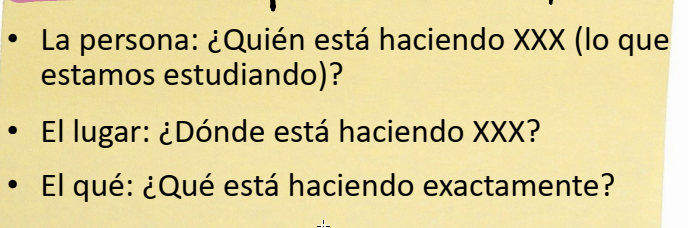
\includegraphics[scale=.3]{Untitled 1.png}}
  \end{figure}
  \item \textbf{Detallado}: Más específico.
  \begin{figure}[H]
    \ffigbox[\FBwidth]
    {\caption{Estructura de observación detallada}}
    {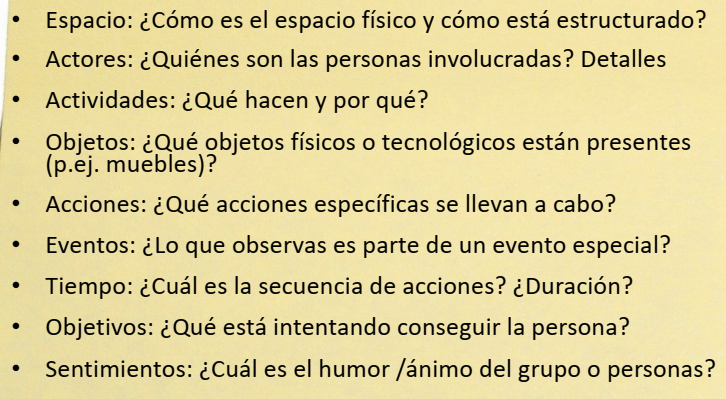
\includegraphics[scale=.25]{Untitled 2.png}}
  \end{figure}
\end{itemize}


\textbf{Grado de participación:} Infiltrado (Activo, participa el
observador en primera persona, difícil disociar participante y
observador) o Ajeno (Pasivo, normalmente en el lab).

\textbf{Planificación y realización:}

\hspace{0pt} Atención equilibrada a participantes.

\hspace{0pt} \textbf{Re-focus}: a medida que surgen aspectos
relevantes.

\hspace{0pt} Actividad intensa, puesto que se anota durante
observaciones y al final del día.

\textbf{Etnográficas}:

\hspace{6mm} Entendimiento detallada, con matices.

\hspace{6mm} \textbf{Rol}: participant observer, activo.

\hspace{6mm} Observaciones directas+entrevistas, cuestionarios, estudios
de artefactos.

\hspace{6mm} Importante, llevar mente abierta, naïve.

\hspace{6mm} \textbf{Datos}: Que hace y dice la gente.

\hspace{6mm} \textbf{Recogida datos}: Notas de campo, documentos,
fotos,\ldots{}

\textbf{Técnicas etnográfica:}

\hspace{6mm} \textbf{Investigación contextual}: Mezcla entrevista y observación. Van haciendo cosas y comentando que hacen.

\hspace{6mm} \textbf{Rol}: activo, modelo de aprendiz.

\hspace{6mm} \textbf{Entrevista contextual}: Observación, discusión y
reconstrucción de eventos pasados.

\hspace{6mm} \textbf{4 principios:} contexto, relación, interpretación y
foco.

\hspace{6mm} \textbf{Recogida datos:} Anotación, grabaciones de audio y
video. Anotaciones al final de las sesiones.

\textbf{Directivas en espacio controlado}

En el laboratorio, más formal y más control, se sigue un protocolo.

Más intrusivo, van a un espacio controlado.

\textbf{Ventajas}: Control de variables.

\textbf{Desventajas}: Pretensión y situación artificial.

\textbf{Foco}: Acciones y comportamientos concretos.

\textbf{Datos}: Video, fotografías, anotaciones.

Hay que tener en cuenta cómo gestionar el equipo.

\textbf{Técnicas}:
\begin{itemize}
  \item \textbf{Think Aloud:} Usuario piensa en voz alta a la vez que
  actúa, lo que nos permite entender lo que piensa y sus modelos mentales
  y expectativas.
  \item \textbf{Diarios:} Los participantes documentan su experiencia.
  
  Auto-documentación de participantes, de forma regular.

  \textbf{Ventajas}: Lo hacen ellos, no requiere mucho tiempo
  de investigadores. Menos logística, es un diario.

  \textbf{Desventajas}: Depende plenamente de los
  participantes, es difícil para los usuarios seguirlo haciendo.
  \item \textbf{Experience Sampling Method (ESM):} Muy parecido al
  diario. Con prompts en momentos concretos determinados por tiempo o
  eventos. Invitan a la acción inmediata.
  \item \textbf{Logs de Interacción:} Software en un dispositivo
  que captura lo que hacen los usuarios para posterior análisis.     Se combina con otras fuentes de datos.

  
    \textbf{Captura}: clics, key press, tiempo empleado.

    \textbf{Ventajas}: No intrusivo.

    \textbf{Desventajas}: Aspecto ético.

    \textbf{Logística}: Herramientas de visualización.
\end{itemize}

\textbf{Elegir una técnica:} No hay una adecuada para todos los casos.
Depende de muchos factores: proyecto, objetivo, usuarios.

\hspace{0pt} Lo mejor es utilizar triangulación, combinar técnicas.

\chapter{Tema 3: Análisis de Estudios de
Campo}

Es importante \textbf{tener evidencias de cómo es realmente el contexto,
no solo suposiciones (assumptions) y verdades no fundadas (claims)},
para esto debemos hacer una buena elección de técnicas de investigación.
Caer en este problema es frecuente, lo importante es saber que no son
verdad.

En esta fase buscamos definir unas técnicas para concretar el contexto
de diseño y saber más, todavía no buscamos la solución.

\textbf{El análisis depende:}

Del \textbf{objetivo} de tu trabajo de campo.

De las \textbf{técnicas} de investigación y recogida de datos.

De tus \textbf{datos} obtenidos con esas técnicas elegidas.

\textbf{Posibles objetivos:}

Entender a los usuarios, es importante diferenciar entre usuario y otros
stakeholder (parte interesada).

Entender actividades, objetos involucrados, espacio de la interacción y
posibles problemas y fricción.

\textbf{Tipos de análisis:} no tiene por qué coincidir con el tipo de
datos.

\begin{itemize}
\item
  \textbf{Cuantitativos}: Proporción, porcentaje, medias\ldots{}
\item
  \textbf{Cualitativos}: Temas emergentes y patrones, impresiones y
  reacciones prominentes\ldots{}

  Los datos deben ser rigurosos y precisos, expresado numéricamente,
  evitando interpretaciones, para poder medir.
\end{itemize}

\section{Tipos de Datos y
Análisis}

\begin{itemize}
\item
  \textbf{Entrevistas}:

  \textbf{Datos}: Notas y grabaciones.

  \textbf{Tratamiento}: Transcripciones y anotaciones extendidas.

  \textbf{Preguntas cerradas:} normalmente cuantitativos.

  \textbf{Preguntas abiertas:} principalmente cualitativo, pero también
  cuantitativo.

  \newpage

\item
  \textbf{Cuestionarios}:

  \textbf{Datos}: Respuestas.

  \textbf{Tratamientos}: Filtrado de datos.

  \textbf{Preguntas cerradas:} normalmente cuantitativos.

  \textbf{Preguntas abiertas:} principalmente cualitativo, pero también
  cuantitativo.
\item
  \textbf{Observaciones}:

  \textbf{Datos}: Muy ricos; notas, logs y grabaciones.

  No es un análisis sencillo, hay muchos datos y debemos equilibrar.

  \textbf{Tratamiento}: Sincronizar fuentes, anotaciones extendidas,
  transcripciones, citas, fragmentos de acciones o interacciones.

  \textbf{Análisis}: según el tipo de datos.

  \begin{itemize}
  
  \item
    \textbf{Cualitativo}: Anotaciones, grabaciones\ldots{}
    
    \item
      \textbf{Cuantitativo}: logs, grabaciones\ldots{}
  \end{itemize}
\end{itemize}

\section{Análisis Cualitativo}

Se identifican en el proceso de recogida de datos.

\subsection{Categorización de
datos}

Anotaciones, entrevistas, transcripciones, se pueden analizar con
distinta granularidad

\begin{itemize}

\item
  \textbf{Gruesa}: Identificación temas, a nivel general.
\item
  \textbf{Fina}: A nivel de palabra, más detallado.
\end{itemize}

\textbf{Esquema de categorización:}

\begin{itemize}

\item
  \textbf{Bottom-up}: De los datos hacia lo general.
\item
  \textbf{Top-down (deductivo)}: esquema establecido con anterioridad
  (teoría, métodos), de lo general hacia los datos.
\item
  Mezcla
\end{itemize}

Importante el rigor, el esquema de categorización tiene que ser fiable y
debe haber concordancia de los distintos evaluadores.

\textbf{Comprobación de nivel de discrepancia}: Coeficiente kappa de Cohen, el
nivel de acuerdo que hay. Si es bajo, mal entrenamiento y problemas en
el esquema de categorización.

\textbf{Técnica:} Content Analysis o \textbf{Análisis de contenido}

Se utiliza para cualquier tipo de documentos y ``textos'' (video,
periodista, citas\ldots)

Es una técnica de \textbf{conteo de ocurrencias}, ya sea temas y
categorías como de palabras clave.

\textbf{Descripción cuantitativa, objetiva, y sistemática del
contenido.}

Cuantifica el contenido en términos de categorías.

\subsection{Identificación de patrones y
temas}

Emergen a medida que te familiarizas con los datos.

Los objetivos del estudio orientan el foco de temas y patrones.

\subsection{Affinity diagram o Diagrama de
afinidad}

\textbf{Organización de notas/ideas/información} según una jerarquía por
similitud.

Es un proceso inductivo, que surge de un flujo de información y se
agrupa, bottom-up.

\textbf{Proceso}:

\begin{enumerate}
\def\labelenumi{\arabic{enumi}.}

\item
  \textbf{Codificación abierta u Open coding}: \textbf{Desgranar los
  datos} en partes discretas, etiquetas.
\item
  \textbf{Codificación axial o Axial coding:} \textbf{Agrupación} de las
  notas por similitud.
\item
  \textbf{Conexión}: De las categorías y etiquetas.
\item
  Creación de \textbf{categorías globales.}
\item
  \textbf{Revisión de datos} con base en estas categorías globales.
\end{enumerate}

Generación de conocimiento y síntesis, para extraer conclusiones.

Se sacan requisitos y necesidades, y se concreta el contexto de diseño.

\subsection{Análisis de Situaciones
clave}

Centrado en comportamientos clave por su impacto:

\begin{itemize}

\item
  \textbf{Critico}: para el desarrollo de la actividad que se estudia.
\item
  \textbf{Deseable}: Impacto positivo.
\item
  \textbf{Indeseable}: Impacto negativo
\end{itemize}

Hay que identificar incidentes significativos por parte de los usuarios
(entrevistas, retrospectiva) y por los propios investigadores
(observación directa, video análisis). Nos permite identificar factores
contextuales, elementos y aspectos clave determinantes de acción,
experiencia\ldots{}

\subsection{Conversation Analysis o Análisis de la
Conversación}

De etnometodología, cómo interactúa la gente y dinámicas de interacción.

\textbf{Microanálisis}: Como se desarrolla la conversación, secuencia y
estructura de la conversación.

Sin suposiciones, ni conjeturas. Búsqueda de patrones

Como la gente se coordina, se entiende, actúa conjuntamente.

\subsection{Video Analysis \& Interaction
Analysis}

Micro o macro.

\textbf{Macro}: Idea general, una primera pasada.

Decisión de elementos clave: momentos o incidencias críticas.

\textbf{Análisis en profundidad}: Descripción de lo ocurrido, con
palabras claves y pantallazos.

\textbf{Herramientas}: Manual, hoja de cálculo o software específico.

\section{Análisis Cuantitativo}

Expresado en forma \textbf{numérica}. Magnitud, cantidad, tamaño, grado,
orden\ldots{} de atributos de participantes.

Compila, ordena, resume, y presenta datos para permitir interpretaciones
posteriores.

\textbf{Organizar los datos, en una estructura estándar}. Filas: sujetos. Columnas: variables.

\textbf{Tipo de variables:}

\begin{itemize}

\item
  \textbf{Cualitativas}: No operaciones aritméticas.

  \begin{itemize}
  
  \item
    \textbf{Ordinales}: Siguen un orden o secuencia. Ej: Meses de año.
  \item
    \textbf{Categóricos}: No siguen un orden. Ej: Estado civil.
  \end{itemize}
\item
  \textbf{Numéricas}: Operaciones aritméticas.

  \begin{itemize}
  
  \item
    \textbf{Discretos}: Valores enteros. Ej: Edad.
  \item
    \textbf{Continuos}: Valores en un intervalo. Ej: Sueldo.
  \end{itemize}
\end{itemize}

\textbf{Análisis de Datos numéricos:}

\begin{itemize}

\item
  \textbf{Medidas de tendencia central:}

  \begin{itemize}
  
  \item
    \textbf{Media}: Promedio.

    \begin{itemize}
    
    \item
      \textbf{Mediana}: El punto central.
    \item
      \textbf{Moda}: Valor más frecuente.
    \end{itemize}
  \end{itemize}
\item
  \textbf{Medidas de dispersión}: Variabilidad de una distribución
  respecto a una medida.

  \begin{itemize}
  
  \item
    \textbf{Desviación típica}: Desviación con la media.

    \begin{itemize}
    
    \item
      \textbf{Rango R}= Max-Min.
    \item
      \textbf{Desviación con la mediana}: Cuartiles.
    \item
      \textbf{Rango intercuartílicos}, IQR: Q3-Q1
    \end{itemize}
  \end{itemize}
\end{itemize}

\section{Tabla de frecuencia}

\begin{figure}[H]
	\ffigbox[\FBwidth]
	{\caption{Ejemplo de Tabla de frecuencias}}
	{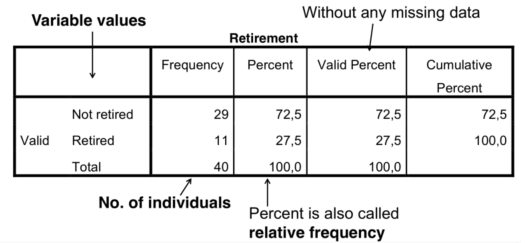
\includegraphics[scale=.5]{Untitled 3.png}}
\end{figure}

\textbf{Datos categóricos.}

Los datos numéricos con variables continuas, y discretas con muchos
valores pueden ser inmanejables, para solventarlo:

\begin{itemize}

\item
  Dividir el rango en clases del mismo tamaño y sin solapamientos.
\item
  Nueva tabla de frecuencias.
\item
  Facilita representación gráfica posterior.
\end{itemize}

\section{Gráficos Estadísticos}

Representación visual de datos estadísticos.

\textbf{Útil} para captar la atención, presentación de información
sencilla, clara y precisa, facilita comparación de datos, destaca
tendencias y diferencias, e ilustrativos.

\subsection{Boxplot o Diagrama de cajas y
bigotes}

Para medidas de tendencia central y dispersión.

\begin{figure}[H]
	\ffigbox[\FBwidth]
	{\caption{Ejemplo de Boxplot}}
	{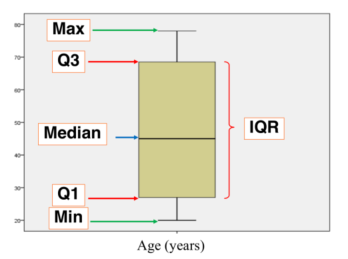
\includegraphics[scale=.5]{Untitled 4.png}}
\end{figure}

Visualiza medidas de desviación con la mediana:

\begin{itemize}

\item
  \textbf{Tres cuartiles}: Q1, Q2, Q3.
\item
  \textbf{Caja}: Q1 y Q3.
\item
  \textbf{Mediana}.
\item
  \textbf{Bigotes}: mínimo y máximo.
\end{itemize}

\section{Gráficos para
Distribuciones}

\subsection{Gráfico de barras}

\begin{figure}[H]
	\ffigbox[\FBwidth]
	{\caption{Ejemplo gráfico de barras}}
	{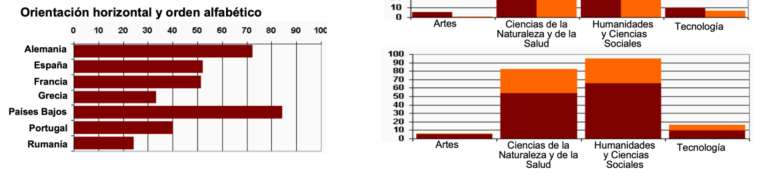
\includegraphics[scale=.5]{Untitled 5.png}}
\end{figure}

Frecuencias de una \textbf{variable cualitativa o discreta}. Sencillo,
agrupado y apilado.

La altura indica la frecuencia o porcentaje y las barras son
\textbf{categóricas}, no valores numéricos.

\textbf{Útil}: Comparar magnitudes.

\textbf{Tipos}: Verticales u horizontales.

\subsection{Polígono de
Frecuencias}

Visualización de frecuencias de cada una de las categorías.
\begin{figure}[H]
	\ffigbox[\FBwidth]
	{\caption{Ejemplo de Polígono de frecuencias}}
	{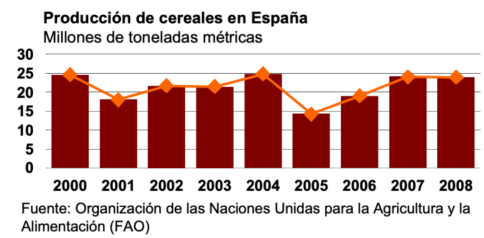
\includegraphics[scale=.5]{Untitled 6.png}}
\end{figure}

\subsection{Histograma}

\begin{figure}[H]
	\ffigbox[\FBwidth]
	{\caption{Ejemplo de Histograma}}
	{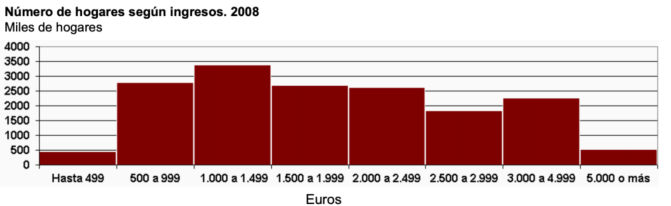
\includegraphics[scale=.4]{Untitled 7.png}}
\end{figure}
Representa las frecuencias de una \textbf{variable cuantitativa
continua.}

Área de la barra es la frecuencia y el eje son intervalos de variable
continua.

\subsection{Gráfico de sectores}
\begin{figure}[H]
	\ffigbox[\FBwidth]
	{\caption{Ejemplo de Gráfico de sectores}}
	{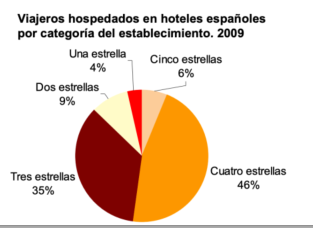
\includegraphics[scale=.5]{Untitled 8.png}}
\end{figure}

Representación circular de las frecuencias relativas.

Variable cualitativa o discreta, se muestran en porcentajes.

Útil: Cuando hay pocas categorías.

\subsection{Gráfico de líneas}
\begin{figure}[H]
	\ffigbox[\FBwidth]
	{\caption{Ejemplo de Gráfico de líneas}}
	{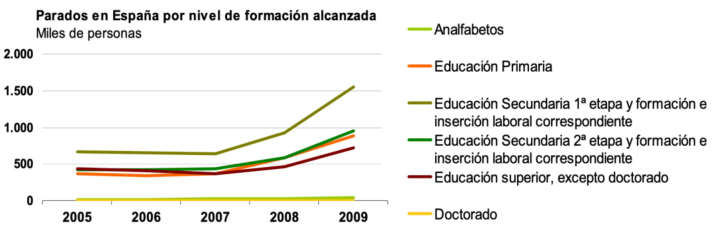
\includegraphics[scale=.5]{Untitled 9.png}}
\end{figure}

Representa relaciones entre dos variables.

Una o varias variables.

Útil para ver tendencias.

\subsection{Gráfico de
Dispersión}

\begin{figure}[H]
	\ffigbox[\FBwidth]
	{\caption{Ejemplo de Gráfico de dispersión}}
	{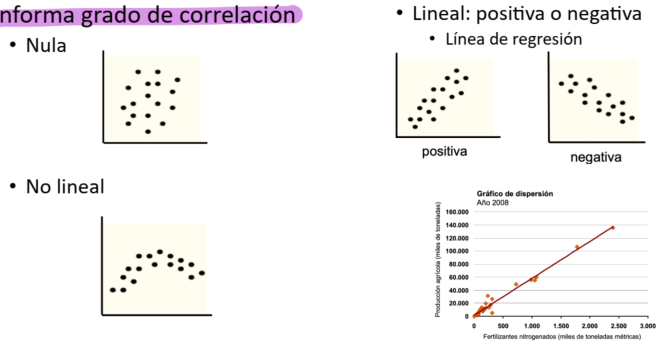
\includegraphics[scale=.4]{Untitled 10.png}}
\end{figure}

Relación entre dos variables ene ejes cartesianos e informa del grado de
correlación.

\section{Resultados}

Requiere habilidad, esfuerzo y trabajo.

Distintas maneras de presentar el material

\textbf{Depende}:

\begin{itemize}
\item
  Del objetivo de tu trabajo de campo
\item
  De tus técnicas de investigación y recogida de datos
\item
  De tus datos obtenidos
\item
  Del análisis realizado
\item
  De la audiencia.
\end{itemize}

\textbf{Propósitos finales:}

\begin{itemize}
\item
  Derivar requisitos, necesidades, design drives.
\item
  Evaluar un producto o en desarrollo.
\end{itemize}

\textbf{Múltiples representaciones}: gráficas, tablas, descripciones
textuales, temas, categorías\ldots{}

\begin{itemize}
\item
  Presentar los resultados.
\item
  Como background o evidencia de conclusiones.
\item
  Para dar rigor, poner el material raw a modo de anexo.
\end{itemize}

\textbf{Tipos}: Resúmenes, Anotaciones rigurosas o Stories.

\chapter{Tema 4: Empezando el proceso de
diseño}

\textbf{Interpretación y transformación de los resultados} del análisis
en requisitos y directrices de diseño. Se pasa de usuarios a personas y
se traza el estado deseado.

Los análisis iniciales antes de interpretar y transformar hay que
tenerlos representado de una manera adecuada, volviéndolos a analizar,
algunos métodos son los siguientes.

\section{Resúmenes}

El objetivo es tener una \textbf{visión general, un resumen general.} Se
trabaja con datos cualitativos, cuantitativo y mixtos.

Se pueden emplear \textbf{múltiples representaciones} como gráficas,
tablas, temas o categorías, para facilitar el seguimiento de los datos.
Van \textbf{acompañados de citas, anécdotas, imágenes o videos para que
sea más ilustrativo y presentar evidencias empíricas.}

\section{Stories}

Storytelling o narraciones, \textbf{manera intuitiva de comunicación de
ideas y experiencias}. Muy usadas en IxD como base para el diseño, se
itera el proceso y se mejora el producto.

Extraídas de anécdotas reales de los usuarios (contadas en entrevistas o
cuestionarios) o de construcciones en base a resultados (observaciones,
encuestas).

Es importante \textbf{especificar procedencia y veracidad,} para dar
validez a las historias.

Son útiles para ilustrar otro tipo de prestaciones de datos,
proporcionar evidencias y aumentar la credibilidad, y para inspirar el
diseño.

\section{Notaciones}

\textbf{Aspectos clave} (necesidades, aspiraciones, expectativas) del
contexto de diseño actual o del diseño futuro que se busca.

Se basan en deseos y necesidades actuales y objetivos de usabilidad y
UX.

Es importante entender el contexto de diseño para proceder de esta
manera, están prefijadas por el proyecto o se producen durante el
proceso de diseño.

\subsection{Notaciones informales}

\textbf{No hay una sintaxis o estructura establecida}, es más abierta
por lo que se puede producir ambiguos.

Mismos aspectos/dimensiones que las notaciones rigurosas.

\textbf{Ventaja}: Inspiran más y permiten innovar, al no ser tan
rígidos.

\textbf{Desventaja}: No son tan preciso y no siguen de guía

\subsection{Notaciones rigurosas o establecidas}

\textbf{Sintaxis y semántica establecidas.}

Tienen una estructura clara.

\textbf{Ventajas}: Guía de una manera más clara de que mirar en cuanto a
conclusiones, y son más precisos.

\textbf{Desventajas}: No son flexible y no permiten la innovación.

\subsection{Requisitos}

\textbf{Declaración que describe de manera clara, concisa y especifica
aspectos y cualidades clave del producto}, que debería hacer y cómo, en
que entorno se va a usar, por quien y como.

No es una lista de features (características).

\textbf{Características}: Específicos (no ambiguos y claro), correctos,
consistentes y verificables.

Lo importante es que los requisitos sean: Medibles, Específicos y bien documentados (vengan de una necesidad del usuario)

\subsection{Requisitos y directrices de diseño}

Se \textbf{discuten, refinan, aclaran y revisan de manera iterativa.}

No se pueden aislar de otras actividades de diseño, \textbf{ambas están
ligadas a las actividades de diseño} y estas a ellos.

Base para empezar a diseñar, \textbf{no son rígidos} por ello se itera
de manera continuada, pero no deben tampoco cambiar radicalmente sin
motivo.

Son importante porque ayudan a \textbf{evitar que un error se prolongó
en el proceso y nos resulte más caro} resolverlo. Los errores se pueden
producir por: Falta de entendimiento con los stakeholders, análisis
deficiente o unas directrices de diseño pobres.

\subsection{Tipos}

\textbf{Ingeniería de Software}: Funcionales y No funcionales.

Las \textbf{7 dimensiones de Gottesdiener y Gorman}: Usuario, Interfaz,
Acciones, Datos, Control, Ambiente (espacio) y Calidad.

\textbf{Espacial/Ambiental}: Espacio físico (luz, humedad, ruido o que
hay), espacio social (usado por una persona o muchas, si es compartido o
individual) y espacio tecnológico (tecnología necesario y limitaciones).

\textbf{Características de usuarios}: Edad, experiencia previa,
circunstancias personales, capacidades físicas, nos permite sacar
distintos requisitos.

\textbf{Objetivos de usabilidad}: Eficiencia, eficacia, satisfacción,
facilidad de aprendizaje con la que unos usuarios determinados alcanza en
un contexto determinado un objetivo concreto.

\textbf{Objetivos de experiencia de usuarios:}

\begin{itemize}

\item
  Percepciones y respuestas resultado del uso y/o anticipación de uso de
  un producto, sistema o servicio.
\item
\textbf{Incluye}: emociones, creencias, preferencias, percepciones, respuestas
  físicas y psicológicas, etc.
\item
\textbf{En definitiva}: Aspectos clave de la experiencia de usuarios/as al
  interactuar con un producto, servicio, entorno o establecimiento
  Algunos aspectos: usabilidad, funcionalidad, estética (experiential
  quality),contenido, el ``look \& feel,'' y el atractivo sensorial y
  emocional. El cómo se siente
\end{itemize}

McCarty \& Wrigth proponen \textbf{4 hilos claves} de una UX integral

\begin{itemize}

\item
\textbf{Sensual thread:} Aspectos sensoriales y viscerales.
\item
\textbf{Emotional thread:} Emociones.
\item
\textbf{Compositional thread:} Parte narrativa de una experiencia.
\item
\textbf{Spatio-temporal thread:} Espacio y tiempo en el que se desarrollan
  nuestras experiencias y que afectan como las vivimos.
\end{itemize}

Ayudan a pensar en la relación entre la tecnología y la experiencia.

\newpage

\section{Atomic Requirements Shell de Volere (Robertson and
Robertson, 2014)}

Define una plantilla de campos que deben tener los requisitos. Framework
general de requisitos no específicos de IxD.
\begin{figure}[H]
	\ffigbox[\FBwidth]
	{\caption{Atomic Requirements Shell de Volere}}
	{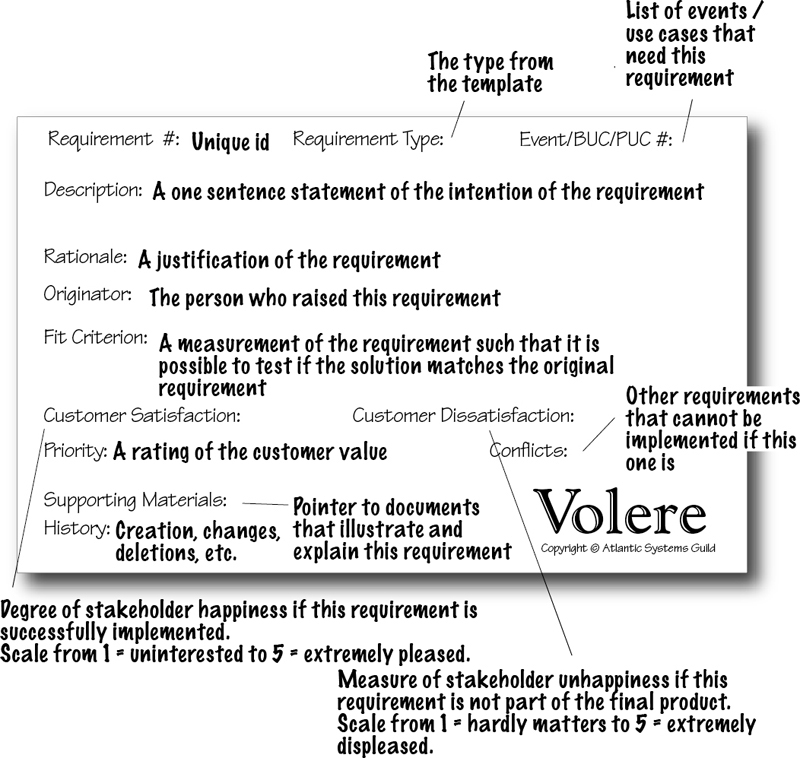
\includegraphics[scale=.4]{2_9_volere_snow_card_alt.jpg}}
\end{figure}

\section{User Stories}

Sirven para \textbf{capturar lo que el producto tiene que hacer e iniciar
una conversión entre stakeholders.}

Muy usadas \textbf{en desarrollo ágil} de software y producto, para
planificar los sprints.

Bloques o unidades de funcionalidades (perspectivas de los usuarios) y
objetivos no funcionales (usabilidad y UX).

\textbf{Consiste en:} descripción, estimación de tiempo, test para
verificación.

\textbf{Epics}: User story complejo, que requiere semanas o meses de
implementación, y se divide en otros más pequeño.

\begin{itemize}

\item
  Del tipo: Yo como \textless\textgreater{} quiero
  \textless\textgreater{} para \textless\textgreater{}
\end{itemize}

\textbf{Task o tareas}: User stories más pequeños de otra más grande.

Se suelen representar como tarjetas, para que \textbf{no quepa mucha
información a propósito}, pero hoy en día hay software específico.

\section{Personas y Scenarios}

Se utilizan para \textbf{transmitir la visión y el propósito de un
producto.}

Suelen ir juntas, funcionan como \textbf{guías para el diseño y
desarrollo} en todas las etapas del UCD.

Se utilizan detalles realistas sobres los usuarios actuales o futuros.

\textbf{Diferencias}:

\begin{itemize}

\item
  Ambos usan la narrativa.
\item
  \textbf{Error común}: mezclar detalles de la persona y del escenario.
\item
  \textbf{Persona}: Caracteriza al usuario \textbf{típico}.
\item
  \textbf{Escenario}: Describe una \textbf{situación o momento de esa
  persona}, usando un producto o intentando conseguir un objetivo.
\end{itemize}

\subsection{Personas (Cooper, 1999)}

\textbf{Descripciones detalladas del usuario típico de un producto.}

No es un usuario concreto. No inventado, usando datos empíricos.

Son \textbf{importantes los detalles para dar vida a las personas} y
poder visualizarlos como usuarios reales.

Se crean normalmente varias personas, una principal que representa una
sección amplia de los usuarios.

Ayudan a la toma de decisiones de diseño y a recordar quien es la gente
que va a usar el producto, \textbf{pensado que haría una persona en esa
situación.}

\textbf{Incluye datos relevantes}: Nombre, foto, datos personales, sus
objetivos, actitudes, aptitudes y detalles relacionados con el tipo de
producto a desarrollar. Aunque hay que equilibrar la información general
y especifica.

\subsection{Scenarios/Escenarios}

\textbf{Descripción narrativa informal.} Describe actividades o tareas
de usuarios y sus objetivos

Permite exploración y discusión acerca de contexto, necesidades, y
requisitos.

No incluye tecnología necesariamente, depende de la fase del proceso.

\textbf{Vocabulario cotidiano, cercano a todos los interesados.}

Permite identificar las partes interesadas, los artefactos involucrados,
el contexto de los usuarios, sus problemas, necesidades, etc.

\textbf{Ejemplos}:

\begin{itemize}

\item
  \textbf{Descripción de un escenario o situación existente}: Es clave
  para entender las prácticas y acciones de los usuarios. Explorar las
  limitaciones, contextos, pain points, facilitadores, etc. Ayudan a
  materializar requisitos.
\item
  \textbf{Descripción de un escenario o situación con una posible
  tecnología futura}: Describe una situación de uso, pone de manifiesto
  necesidades de los usuarios y posibles aspectos de diseño.
\item
  \textbf{Descripción de una función del sistema futuro}: Describe una
  función e incluye a dos personas. Pone de manifiesto suposiciones,
  expectativas y situaciones en las que se pueden ver los usuarios.
  Ayuda a traducir en requisitos, como un requisito ambiental.
\end{itemize}

Se desarrollan después del análisis del trabajo de campo, para explicar
o discutir aspectos clave de los objetivos de los usuarios en acción. No
capturen todos los objetivos, ni se relaciona con todos los requisitos.

Se centran en el detalle y la riqueza.

\section{Use Cases o Casos de Uso}

\textbf{Describe la interacción de manera más precisa}, no tanto el
contexto.

Se centra en \textbf{requisitos funcionales y en objetivos de usuarios} pero
con \textbf{énfasis en la interacción} usuario-producto.

No son lo mismo que las user stories, son más dirigidas a la
interacción.

Describe \textbf{paso a paso y de manera detallada} a la interacción.

Útil para pensar acerca de la interacción y para capturar nuevos
requisitos (enriquece requisitos básicos).

\textbf{Varios estilos:}

\begin{itemize}
	\item \textbf{Estilo 1 Essential Use Case Constantine and Lockwood (1999)}
		\begin{itemize}
			\item División en tareas del usuario y del producto. Solo menciona tareas.
			\item Se representa como Intención usuario y Responsabilidad del sistema. No mucho acerca de la interaccione exacta.
		\end{itemize}
	\item \textbf{Estilo 2: Mas detallado y especifico}
		\begin{itemize}
			\item Captura el objetivo del usuario cuando interactúa con el producto. Se describe la interacción de una manera más guiada y natural.
			\item Se muestras distintos cursos (maneras), uno principal que es la más común, y otros alternativos por si se produce un error o hay otra vía para alcanzar el objetivo.
		\end{itemize}
\end{itemize}

\chapter{Tema 5: Diseño y prototipado de la interacción}

\section{Preferred State}
Visión de situación futura, del futuro contexto de diseño. Basado en el contexto de diseño actual, en aspectos que funcionan. Se dice preferred porque queremos que mejor con respecto al actual.

Se utiliza el brainstorming para delinearlo, centrado en posibles soluciones y en aspectos claves del contexto de diseño. Se incluyen también aspectos aspiracionales y cambios.

Para trazar el preferred state, se selecciona una serie de parámetros como directrices de diseño; un par o más, que nos permita definir un estado que queremos alcanzar.

\section{Proceso Iterativo de Diseño}

\begin{figure}[H]
	\ffigbox[\FBwidth]
	{\caption{Double Diamond}}
	{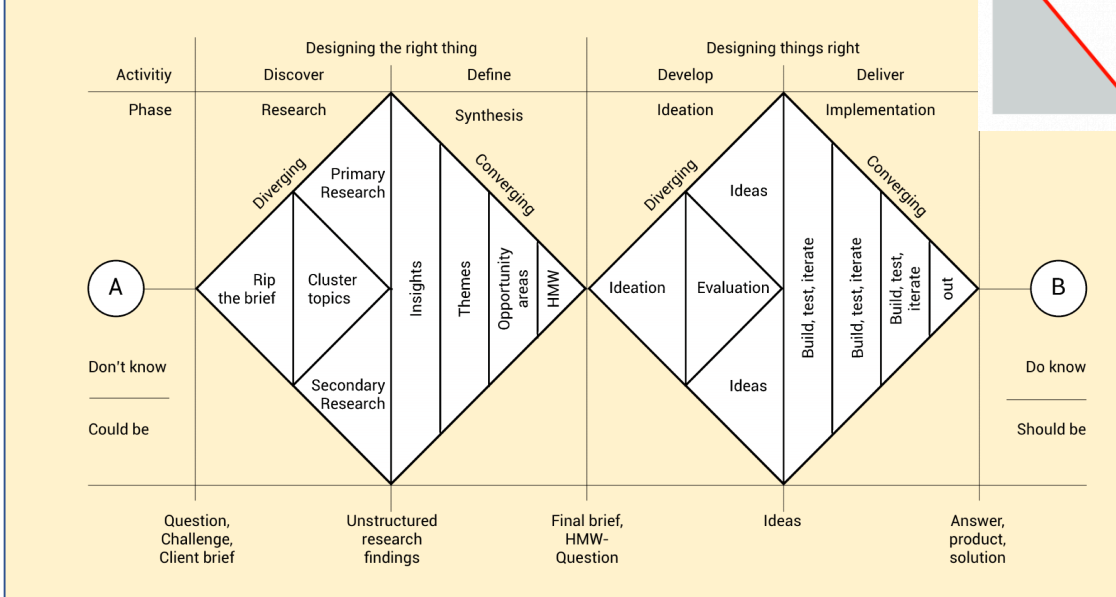
\includegraphics[scale=.4]{2021-03-20 21_09_36-L5.pdf - Foxit Reader.png}}
\end{figure}

Dos tipos de diseño, que están vinculados.
\begin{itemize}
  \item Conceptual, la idea del producto, los aspectos generales. Fase divergente de ideación.
  \item Detalles, aspectos concretos del producto. Fase de convergencia de diseño y desarrollo.
\end{itemize}

\section{Brainstorming}
El objetivo general es obtener una gran cantidad de diferentes ideas, poder definir el problema y objetivos. Cantidad antes que calidad, el objetivo es sacer ideas no analizarlas.

Se realiza en un tiempo acotado y claro, en el que es importante que los participantes puedan aportar ideas.

Es importante que se muy visual, para reconocer cada idea de manera fácil, por eso se utilizan post-its, diagramas, sketches...

\textbf{Reglas del juego:}
\begin{itemize}
  \item Cantidad antes que calidad, ya se filtrará más tarde.
  \item Un post-it es una idea.
  \item No se discuten las ideas, ni se critican, ni se piensa en la viabilidad.
  \item Construir ideas sobre otras.
\end{itemize}

Creatividad e innovación, un consejo es un utilizar facilitadores (prompts) para sacar las ideas, como puede ser ir por temáticas (Temáticos), temporales, ir variando (cambios de foco), que no tengan nada que ver para romper un momento la búsqueda y volver a pensar.

También es importante la fase de análisis y convergencia, en la que se seleccionan, agrupan y clasifican las ideas.

Todo deben quedar documentando para posteriormente analizarlo y que nos sea de utilidad, se pueden usar fotos, post-its, ordenadores, ideas enumeradas, ...

\section{Después de la fase de ideación}

Habremos poblado el espacio de diseño con distintos conceptos, al menos uno por personas en el grupo, cada uno puede que responda a distintos aspectos del contexto de diseño

\textbf{Siguiente pasos:}
\begin{itemize}
  \item Convergencia, nos quedamos con un concepto de diseño por persona.
  \item Pasamos a diseño conceptual con más de Detalles.
  \item Convergencia: selección de UN concepto de diseño que será el que prototipemos.
  \item Prototipado.
\end{itemize}

\section{De Diseño Conceptual a Concreto}
\subsection{Sketch - Boceto}
Primera herramienta de diseño conceptual se usa pronto en el proceso de diseño para proponer, explorar, y comunicar ideas.

Suelen se minimalistas, no contiene todos los detalles. Foco: multiplicidad y abundancia.

\textbf{Ventajas:}
\begin{itemize}
  \item Rápido y oportuno.
  \item Barato y desechable (no debe costar deshacerse de uno)
  \item Ilustrativo, debe permitir tener una primera visión para documentar, compartir, discutir y criticas ideas.
  \item Permite pensar a través de ideas, de manera abierta. Los sketches te responden (talk back), permite recibir feedback sobre la idea de proceso que tenemos y si es posible en este.
\end{itemize}

\subsection{Prototipo vs Sketch}
Son complementarios, no intercambiables.

Los prototipos requieren mayor inversión.

El boceto es para sacar ideas rápido y es más abierto, sin embargo, el prototipo es algo más concreto y cerrado, aunque puede recibir modificaciones.

\subsection{Prototipos}
Manifestación o materialización de un concepto de diseño que nos permite probar y explorar opciones, y comunicar ideas entre diseñadores/as, y otras partes interesadas (incluidos/as usuarios/as).

No es un producto terminado.

Resalta una serie de características y mitiga otras.

Se pasa de diseño conceptual a diseño concreto centrado en detalles, aunque el refinamiento depende del momento en el proceso de diseño.

Compromisos: Horizontal centrado en lo visual, o Vertical centrado en ser funcional.
\subsubsection{Low fidelity - Baja fidelidad}
Muy básicos, permite realizar muchas versiones rápido y barato, para ir mejorandolo.
  
\textbf{Ventajas}
  \begin{itemize}
    \item Herramienta de comunicación muy útil.
    \item Prueba de conceptos.
    \item Revisiones rápidas, se buscará la calidad más adelante.
    \item Mejora del diseño antes del desarrollo.
    \item Permite evaluar múltiples conceptos.
  \end{itemize}

  \textbf{Desventajas}
  \begin{itemize}
    \item No centrado en errores y bugs.
    \item Poca especificidad para el desarrollo.
    \item No para estudios de usabilidad, sino de experiencia de usuario.
    \item Limitaciones en navegación y flujo.
    \item Requiere facilitación, que alguien vaya explicando que es cada cosa y que nos permite.
  \end{itemize}
  
  \subsubsection{Mago de Oz}

  \begin{figure}[H]
    \ffigbox[\FBwidth]
    {\caption{Diagrama Wizard of Oz}}
    {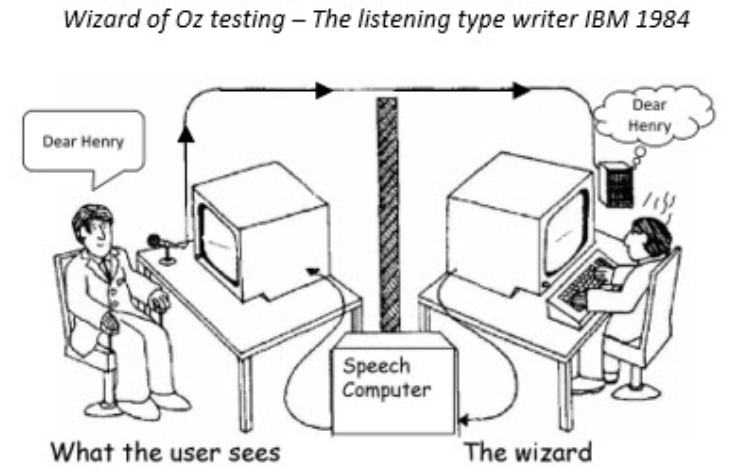
\includegraphics[scale=.4]{2021-03-20 23_48_56-L5.pdf - Foxit Reader.png}}
  \end{figure}

  Alguien simula cómo funciona el sistema mientras se evalúa el prototipo. Centrado en la interactividad y la experiencia. Mas barato que implementar las funcionalidades.

  \subsubsection{High Fidelity - Alta fidelidad}
  Bastante funcionales.

  \textbf{Ventajas}
  \begin{itemize}
    \item Funcionalidad casi completa.
    \item Totalmente interactivos.
    \item Centrados en el usuario.
    \item El esquema de navegación está definido.
    \item Se puede ver y probar algo muy cercano al producto final.
    \item Sirve como herramienta de marketing.
  \end{itemize}

  \textbf{Desventajas}
  \begin{itemize}
    \item Requiere muchos más recursos y tiempo de desarrollo.
    \item Las modificaciones requieren mucho tiempo.
    \item Ineficiente como prueba de conceptos.
    \item Puede confundirse con el producto final.
    \item Expectativas no realistas.
  \end{itemize}

\subsection{Prototipos vs. Wireframes vs. Mockup}
Los Wireframes y Mockups son muy usados en desarrollo web, se diferencian en el objetivo, fase y acabado del diseño.

\textbf{Wireframe:} Coste bajo, fidelidad baja-media. Es una representación visual básica de la interfaz.

\textbf{Mockup:} Coste medio, fidelidad media-alta. Representación más precisa.

\textbf{Prototipo:} Coste alto, fidelidad alta. Está centrado en la interactividad.

\subsection{Wireframes}

\begin{figure}[H]
	\ffigbox[\FBwidth]
	{\caption{Ejemplo Wireframe}}
	{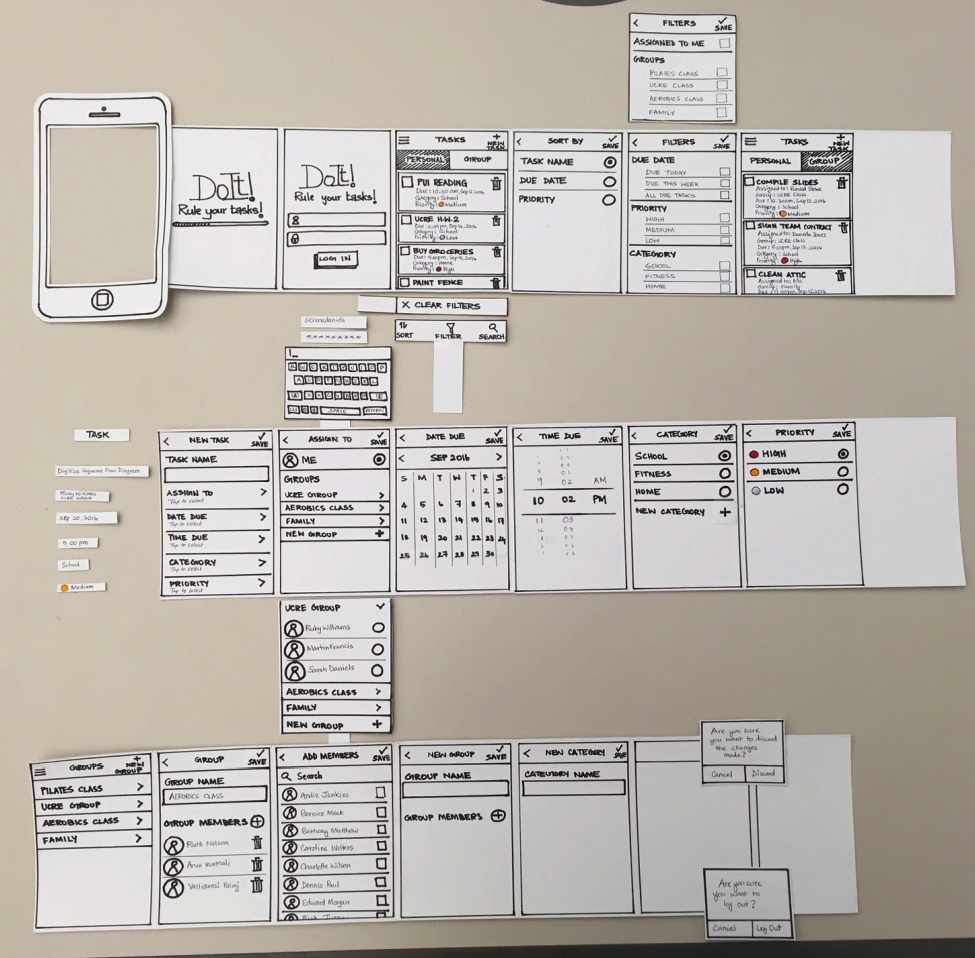
\includegraphics[scale=.4]{2021-03-20 23_51_33-L5.pdf - Foxit Reader.png}}
\end{figure}

Prototipado más básico. Es un prototipo de nivel medio funcional.

Baja fidelidad. La documentación está centrada en la funcionalidad.

A nivel de estructura, contenido principal, la interfaz más básica.
Pantallas claves.

Barato y rápido de hacer.

Normalmente de baja resolución: En papel, cartulinas, bolígrafo, lápices de colores... y en escalas de grises o colores muy básicos, ya que no es lo que importa.

\textbf{Wireflow (wireframes + flowchart):} Cambios pantalla a pantalla, como un storyboard, con distintos niveles de detalle. Centrados en la interactividad.

\subsection{Paper Prototyping + Wizard of Oz}

Es habitual la mezcla de wireframes y Mago de Oz, permite estudios con usuarios.
Se crean las pantallas de un wireflow. Con wireframes de baja resolución.

\textbf{Roles:} 1 Wizard, 1 facilitador y el resto anotando interacciones, controlando cámaras y demás logística.

\subsection{Mockups}
Prototipado de media a alta fidelidad. Muy centrado en la estética para realizar decisiones respecto al color, esquemas, estilo visual, tipografía…

Más costoso de hacer. Se requiere SW específico.

\section{Más allá del prototipado del producto}
\subsection{Storyboard}

\begin{figure}[H]
	\ffigbox[\FBwidth]
	{\caption{Ejemplo Storyboard}}
	{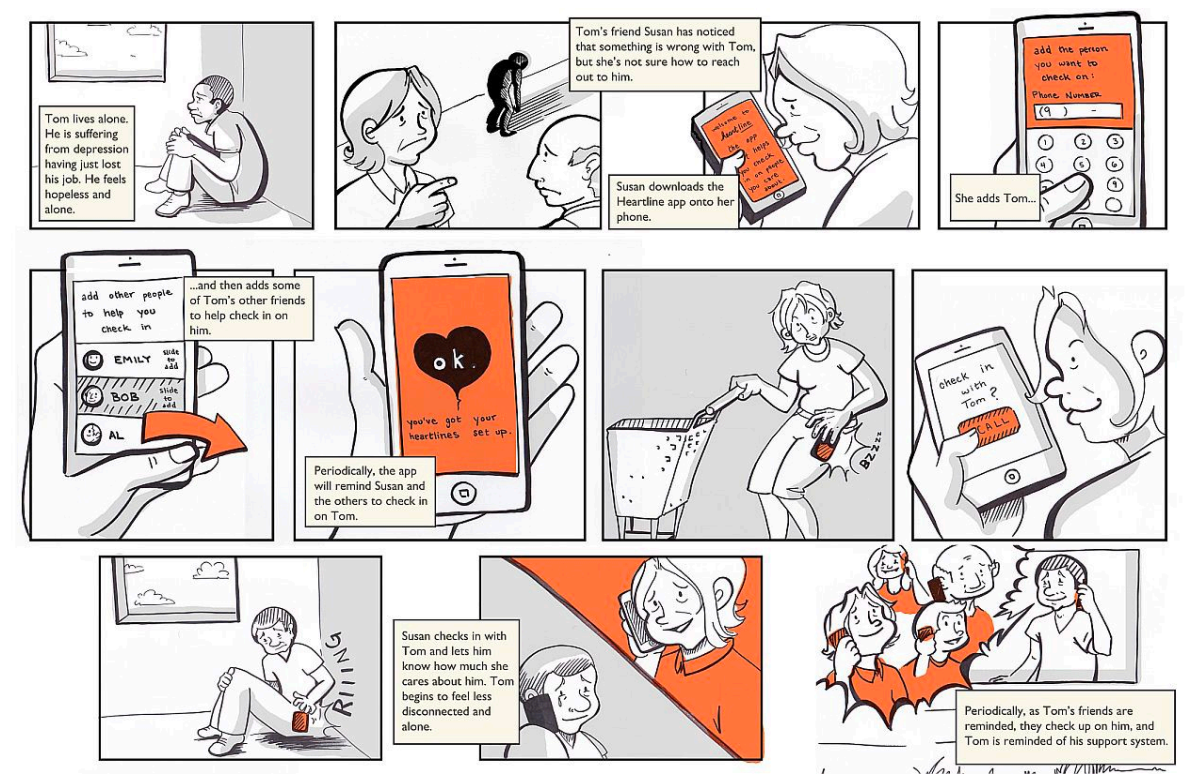
\includegraphics[scale=.4]{2021-03-20 23_53_31-L5.pdf - Foxit Reader.png}}
\end{figure}

Muy visual, influenciado por comics y películas. Ilustraciones secuenciales de acciones o eventos por los que pasa el usuario y el producto para conseguir un objetivo.

\textbf{Objetivo: }
\begin{itemize}
  \item Predecir y explorar cuál va a ser la experiencia de un/una usuario/a con un producto.
  \item Ayudar al equipo de diseño a considerar el escenario y el uso del producto en más detalle.
  \item Obtener feedback de usuarios/as.
\end{itemize}

\textbf{Parte de personas + scenarios:} Centrado en la interacción. Se piensa primero en que aparecerá en las ilustraciones, se hacen primero a bajo detalle y con descripciones de las escenas, después de ver que todo está bien se hacen los dibujos finales con más detalle.

\textbf{Escenas clave:} Problema inicial, Interacción (desarrollo de la situación) y Resolución (beneficio y experiencia final).

\subsection{Técnicas de diseño ”embodied”}
\subsubsection{Embodied Sketching}
Utilizar el cuerpo, acciones, movimientos para el proceso de diseño, la participación física y social. extensión de método de diseño tradicionales como brainstorming, scenarios, personas...

Se utiliza en distintos momentos del proceso de diseño.

\textbf{Objetivos:} Sensibilización, Ideación: Brainstorming (generar ideas con el cuerpo) y Evaluación: Participatory embodied sketching (el usuario participa en el diseño).

\subsection{Sensibilización para entender a usuarios/as y contexto}
\subsubsection{Sensibilización}
Representación, improvisación. Reproducir acciones cotidianas de los/as usuarios/as.

\textbf{Quién:} El equipo de diseño.

\textbf{Técnicas:} Acciones desgranadas, Imágenes congeladas y Representación de “personas”.


\textbf{Forum Theatre}
Se representa una acción y el equipo sugiere cambios u otras condiciones y se vuelve a representar, para ver esa alternativa.

\textbf{Quién:} diseñadores/as, actores/actrices.

\textbf{Técnica:} Escenarios Modificables, Script e improvisación.

\subsection{Sensibilización para inspirar nuevas ideas}
\subsubsection{Sensibilización + Ideación}
\textbf{Brainstorming “in the wild”} “en el campo” “o en el sitio”

Ir al lugar del contexto o un lugar similar para hacer allí el brainstorming ayuda a visualizar.

\textbf{Objetivo:} Condiciones similares, Empatía con los/as usuarios/as, Inmersión física (espacial) y Feedback inmediato

\subsubsection{Sensibilización}
\textbf{Objetivos:}
\begin{itemize}
  \item Sensibilizar a participantes (diseñadores/as, pero también otros/as)
  \item Crear un vocabulario común para el equipo
  \item Inspirar nuevas maneras de pensar
  \item Inspirar ideas nuevas
\end{itemize}

\textbf{Quién:}
\begin{itemize}
  \item Diseñadores/as
  \item Facilitadores/as (expertos/as en actividad de sensibilización)
\end{itemize}

\textbf{Técnicas:}
\begin{itemize}
  \item Participación conjunta en una actividad/experiencia relevante
  \item Exploración activa de recursos y material de diseño
  \item Logística: Props, espacio
  \item Facilitación e instrucción
  \item Actividad de diseño posterior
\end{itemize}

\subsubsection{Bodystorming}
Es ideación utilizando el cuerpo. Se realiza pronto e intervienen diseñadores y facilitadores.

Proceso conducido por acciones clave de la experiencia: embodied core mechanics

\textbf{Objetivo:} poblar el espacio de diseño (design space) a través de sketches de esas mechanics

\textbf{Técnicas:} Como brainstorming e Ideación rápida o más específicas como Uso de props, Propuesta por turnos o Colaboración en la escenificación.

\subsubsection{Ideación, iteración}
\textbf{Strong Prototyping}

\textbf{Técnica:} Fuerte Prototipado de escenarios

\textbf{Quién:} diseñadores/as

\textbf{Objetivo:} Condiciones similares, Empatía usuarios/as, Inmersión física (espacial) y Feedback inmediato

\end{document}
